\documentclass[
  shownotes,
  xcolor={svgnames},
  hyperref={colorlinks,citecolor=DarkBlue,linkcolor=DarkRed,urlcolor=DarkBlue}
  , aspectratio=169]{beamer}
\usepackage{animate}
\usepackage{amsmath}
\usepackage{amsfonts}
\usepackage{amssymb}
\usepackage{pifont}
\usepackage{mathpazo}
%\usepackage{xcolor}
\usepackage{multimedia}
\usepackage{fancybox}
\usepackage[para]{threeparttable}
\usepackage{multirow}
\setcounter{MaxMatrixCols}{30}
\usepackage{subcaption}
\usepackage{graphicx}
\usepackage{lscape}
\usepackage[compatibility=false,font=small]{caption}
\usepackage{booktabs}
\usepackage{ragged2e}
\usepackage{chronosys}
\usepackage{appendixnumberbeamer}
\usepackage{animate}
\setbeamertemplate{caption}[numbered]
\usepackage{color}
%\usepackage{times}
\usepackage{tikz}
\usepackage{comment} %to comment
%% BibTeX settings
\usepackage{natbib}
\bibliographystyle{apalike}
\bibpunct{(}{)}{,}{a}{,}{,}
\setbeamertemplate{bibliography item}{[\theenumiv]}

% Defines columns for bespoke tables
\usepackage{array}
\newcolumntype{L}[1]{>{\raggedright\let\newline\\\arraybackslash\hspace{0pt}}m{#1}}
\newcolumntype{C}[1]{>{\centering\let\newline\\\arraybackslash\hspace{0pt}}m{#1}}
\newcolumntype{R}[1]{>{\raggedleft\let\newline\\\arraybackslash\hspace{0pt}}m{#1}}


\usepackage{xfrac}


\usepackage{multicol}
\setlength{\columnsep}{0.5cm}

% Theme and colors
\usetheme{Boadilla}

% I use steel blue and a custom color palette. This defines it.
\definecolor{andesred}{HTML}{af2433}

% Other options
\providecommand{\U}[1]{\protect\rule{.1in}{.1in}}
\usefonttheme{serif}
\setbeamertemplate{itemize items}[default]
\setbeamertemplate{enumerate items}[square]
\setbeamertemplate{section in toc}[circle]

\makeatletter

\definecolor{mybackground}{HTML}{82CAFA}
\definecolor{myforeground}{HTML}{0000A0}

\setbeamercolor{normal text}{fg=black,bg=white}
\setbeamercolor{alerted text}{fg=red}
\setbeamercolor{example text}{fg=black}

\setbeamercolor{background canvas}{fg=myforeground, bg=white}
\setbeamercolor{background}{fg=myforeground, bg=mybackground}

\setbeamercolor{palette primary}{fg=black, bg=gray!30!white}
\setbeamercolor{palette secondary}{fg=black, bg=gray!20!white}
\setbeamercolor{palette tertiary}{fg=white, bg=andesred}

\setbeamercolor{frametitle}{fg=andesred}
\setbeamercolor{title}{fg=andesred}
\setbeamercolor{block title}{fg=andesred}
\setbeamercolor{itemize item}{fg=andesred}
\setbeamercolor{itemize subitem}{fg=andesred}
\setbeamercolor{itemize subsubitem}{fg=andesred}
\setbeamercolor{enumerate item}{fg=andesred}
\setbeamercolor{item projected}{bg=gray!30!white,fg=andesred}
\setbeamercolor{enumerate subitem}{fg=andesred}
\setbeamercolor{section number projected}{bg=gray!30!white,fg=andesred}
\setbeamercolor{section in toc}{fg=andesred}
\setbeamercolor{caption name}{fg=andesred}
\setbeamercolor{button}{bg=gray!30!white,fg=andesred}


\usepackage{fancyvrb}
\newcommand{\VerbBar}{|}
\newcommand{\VERB}{\Verb[commandchars=\\\{\}]}
\DefineVerbatimEnvironment{Highlighting}{Verbatim}{commandchars=\\\{\}}
% Add ',fontsize=\small' for more characters per line
\usepackage{framed}
\definecolor{shadecolor}{RGB}{248,248,248}
\newenvironment{Shaded}{\begin{snugshade}}{\end{snugshade}}
\newcommand{\AlertTok}[1]{\textcolor[rgb]{0.94,0.16,0.16}{#1}}
\newcommand{\AnnotationTok}[1]{\textcolor[rgb]{0.56,0.35,0.01}{\textbf{\textit{#1}}}}
\newcommand{\AttributeTok}[1]{\textcolor[rgb]{0.77,0.63,0.00}{#1}}
\newcommand{\BaseNTok}[1]{\textcolor[rgb]{0.00,0.00,0.81}{#1}}
\newcommand{\BuiltInTok}[1]{#1}
\newcommand{\CharTok}[1]{\textcolor[rgb]{0.31,0.60,0.02}{#1}}
\newcommand{\CommentTok}[1]{\textcolor[rgb]{0.56,0.35,0.01}{\textit{#1}}}
\newcommand{\CommentVarTok}[1]{\textcolor[rgb]{0.56,0.35,0.01}{\textbf{\textit{#1}}}}
\newcommand{\ConstantTok}[1]{\textcolor[rgb]{0.00,0.00,0.00}{#1}}
\newcommand{\ControlFlowTok}[1]{\textcolor[rgb]{0.13,0.29,0.53}{\textbf{#1}}}
\newcommand{\DataTypeTok}[1]{\textcolor[rgb]{0.13,0.29,0.53}{#1}}
\newcommand{\DecValTok}[1]{\textcolor[rgb]{0.00,0.00,0.81}{#1}}
\newcommand{\DocumentationTok}[1]{\textcolor[rgb]{0.56,0.35,0.01}{\textbf{\textit{#1}}}}
\newcommand{\ErrorTok}[1]{\textcolor[rgb]{0.64,0.00,0.00}{\textbf{#1}}}
\newcommand{\ExtensionTok}[1]{#1}
\newcommand{\FloatTok}[1]{\textcolor[rgb]{0.00,0.00,0.81}{#1}}
\newcommand{\FunctionTok}[1]{\textcolor[rgb]{0.00,0.00,0.00}{#1}}
\newcommand{\ImportTok}[1]{#1}
\newcommand{\InformationTok}[1]{\textcolor[rgb]{0.56,0.35,0.01}{\textbf{\textit{#1}}}}
\newcommand{\KeywordTok}[1]{\textcolor[rgb]{0.13,0.29,0.53}{\textbf{#1}}}
\newcommand{\NormalTok}[1]{#1}
\newcommand{\OperatorTok}[1]{\textcolor[rgb]{0.81,0.36,0.00}{\textbf{#1}}}
\newcommand{\OtherTok}[1]{\textcolor[rgb]{0.56,0.35,0.01}{#1}}
\newcommand{\PreprocessorTok}[1]{\textcolor[rgb]{0.56,0.35,0.01}{\textit{#1}}}
\newcommand{\RegionMarkerTok}[1]{#1}
\newcommand{\SpecialCharTok}[1]{\textcolor[rgb]{0.00,0.00,0.00}{#1}}
\newcommand{\SpecialStringTok}[1]{\textcolor[rgb]{0.31,0.60,0.02}{#1}}
\newcommand{\StringTok}[1]{\textcolor[rgb]{0.31,0.60,0.02}{#1}}
\newcommand{\VariableTok}[1]{\textcolor[rgb]{0.00,0.00,0.00}{#1}}
\newcommand{\VerbatimStringTok}[1]{\textcolor[rgb]{0.31,0.60,0.02}{#1}}
\newcommand{\WarningTok}[1]{\textcolor[rgb]{0.56,0.35,0.01}{\textbf{\textit{#1}}}}
\usepackage{graphicx}
\makeatletter

\definecolor{airforceblue}{rgb}{0.36, 0.54, 0.66}

\usepackage{tikz}
% Tikz settings optimized for causal graphs.
\usetikzlibrary{shapes,decorations,arrows,calc,arrows.meta,fit,positioning}
\tikzset{
    -Latex,auto,node distance =1 cm and 1 cm,semithick,
    state/.style ={ellipse, draw, minimum width = 0.7 cm},
    point/.style = {circle, draw, inner sep=0.04cm,fill,node contents={}},
    bidirected/.style={Latex-Latex,dashed},
    el/.style = {inner sep=2pt, align=left, sloped}
}


\makeatother






%%%%%%%%%%%%%%% BEGINS DOCUMENT %%%%%%%%%%%%%%%%%%

\begin{document}

\title[Lecture 15]{Lecture 15: \\ Overfit \& Cross Validation}
\subtitle{Big Data and Machine Learning for Applied Economics \\ Econ 4676}
\date{\today}

\author[Sarmiento-Barbieri]{Ignacio Sarmiento-Barbieri}
\institute[Uniandes]{Universidad de los Andes}


\begin{frame}[noframenumbering]
\maketitle
\end{frame}

%%%%%%%%%%%%%%%%%%%%%%%%%%%%%%%%%%%

%----------------------------------------------------------------------%
\begin{frame}
\frametitle{Announcements}

\begin{itemize}
  \item Problem Set 3 deadline change to October 15. You {\bf should not} work on the break.
  \item Problem Sets 4, 5, and 6 are up.
  \item Final Project
  \medskip
  \begin{itemize}
    \item First deadline. October 22. 
    \begin{itemize}
     \item This submission should be a brief statement of what you plan to do. 
     \item Max 2 pages.
     \end{itemize}
     \medskip
    \item  Second deadline. Presentations. November 30th, December 2nd, and 3rd.
      \medskip
    \item  Final document. December 10th at 6 pm
  \end{itemize}

\end{itemize}

\end{frame}

%----------------------------------------------------------------------% 

\begin{frame}
\frametitle{Agenda}

\tableofcontents

\end{frame}

%----------------------------------------------------------------------%
\section{Recap}
%----------------------------------------------------------------------%
\begin{frame}[fragile]
\frametitle{Linear Models}

\begin{itemize}

 \item Last class we talked about the linear model

    \begin{align}
    y = X \beta + u
    \end{align}
    
\item We focused on predicting $y$ and the connection to classical econometrics
\medskip
\item In the classical view, the linearity is given and the notion of complexity is somehow easily defined.
\end{itemize}

\end{frame}
%----------------------------------------------------------------------%
\begin{frame}[fragile]
\frametitle{General Models}

\begin{itemize}
\item However, we can think about more general models

\begin{align}
    y = f(X)  + u
    \end{align}

\item where $f$ is some fixed but unknown function of X and u is a mean-zero error which is independent of x
\item  The emphasis here is that this is a statistical model. There is nothing causal in it. In the model, $f$ represents the systematic relationship between X and y and u represents idiosyncratic deviations from this systematic relationship.
\medskip
\item  Note that:
\begin{itemize}
  \item f is not restricted in any way – it can be a completely arbitrary and complex function.
  \item  Predicting $y$ involves \emph{learning} $f$, that is, $f$ is no longer taken as given, as in the classical view. 
  \item It implies an iterative process where initial choices for $f$ are revised in light of potential improvements in predictive performance.
\end{itemize}
  
  

\end{itemize}
\end{frame}
%----------------------------------------------------------------------%
\begin{frame}[fragile]
\frametitle{Supervised Learning}

\begin{align}
    y = f(X)  + u
    \end{align}

\begin{itemize}
\item The problem of learning $y$ based on features $X$ is known as a supervised learning task.
\medskip
\item $y$ supervises the learning.

\item For prediction we don’t care about f itself. We can treat it as a black box, and any approximation $\hat f$ that yields a good prediction is good enough.

\bigskip

\begin{quote}
\centering
Whatever works, works.
\end{quote}


\end{itemize}

\end{frame}
%----------------------------------------------------------------------%
\begin{frame}[fragile]
\frametitle{Supervised Learning}

\begin{itemize}
\item What is ‘what works’, i.e., what is a good prediction?
\medskip
\item  Formally, a supervised learning algorithm takes as an input a loss function and searches for a function $\hat{f}$ within a function class $\mathcal{F}$ that has a low expected prediction loss
\medskip

\item The goal here is to solve something which looks like
\begin{align}
\hat{f}=\underset{f\in\mathcal{F}}{\text{argmin}}\left\lbrace E \left(L(y,f(X) \right) \right\rbrace
\end{align}
\medskip

for some loss function $L$, and for some set of predictors $\mathcal{F}$. 
\medskip
\item Note that here in a function space, so we are solving for a function not a point.



\end{itemize} 

\end{frame}

%----------------------------------------------------------------------%
\begin{frame}
\frametitle{Error Decomposition}

\begin{itemize} 
\item The most common function is the squared error loss $\rightarrow$ MSE
  \medskip
\begin{align}
E \left(L(y,\hat{y}) \right)  &= E(y-\hat f)^2  \\
                 &= E(f-\hat{f})^2 + E(u^2) \\
                 &=\underset{Reducible\,error}{ MSE(\hat f)} +  \underset{Irreducible\,error}{E(u^2)} 
\end{align}

\medskip

  \item There is a lower bound to the accuracy of the best possible prediction for a given $f$, given by the variance of the idiosyncratic error.
  
\end{itemize}

\end{frame}
%----------------------------------------------------------------------%
\section{Overfit}
%----------------------------------------------------------------------%
\begin{frame}[fragile]
\frametitle{Overfit}

\begin{itemize} 
  \item Why don’t we estimate the most flexible function that we can?
\end{itemize}
        \begin{figure}[H] \centering
            \captionsetup{justification=centering}
              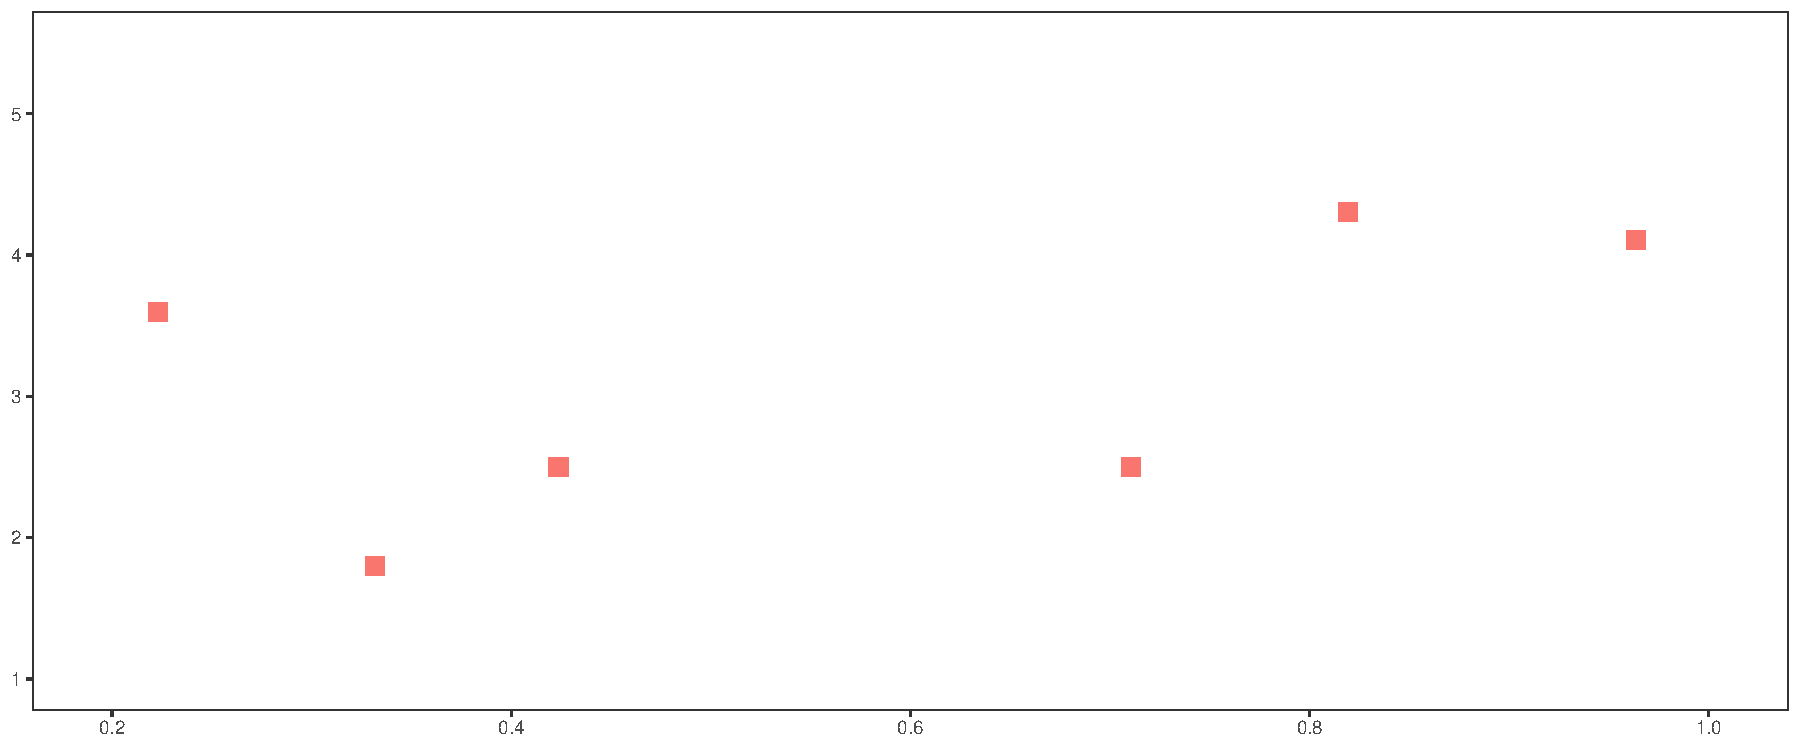
\includegraphics[scale=0.4]{figures/fig_1a.pdf}
 \end{figure}


\end{frame}
%----------------------------------------------------------------------%
\begin{frame}[fragile]
\frametitle{Overfit}

\begin{itemize} 
  \item Why don’t we estimate the most flexible function that we can?
\end{itemize}
        \begin{figure}[H] \centering
            \captionsetup{justification=centering}
              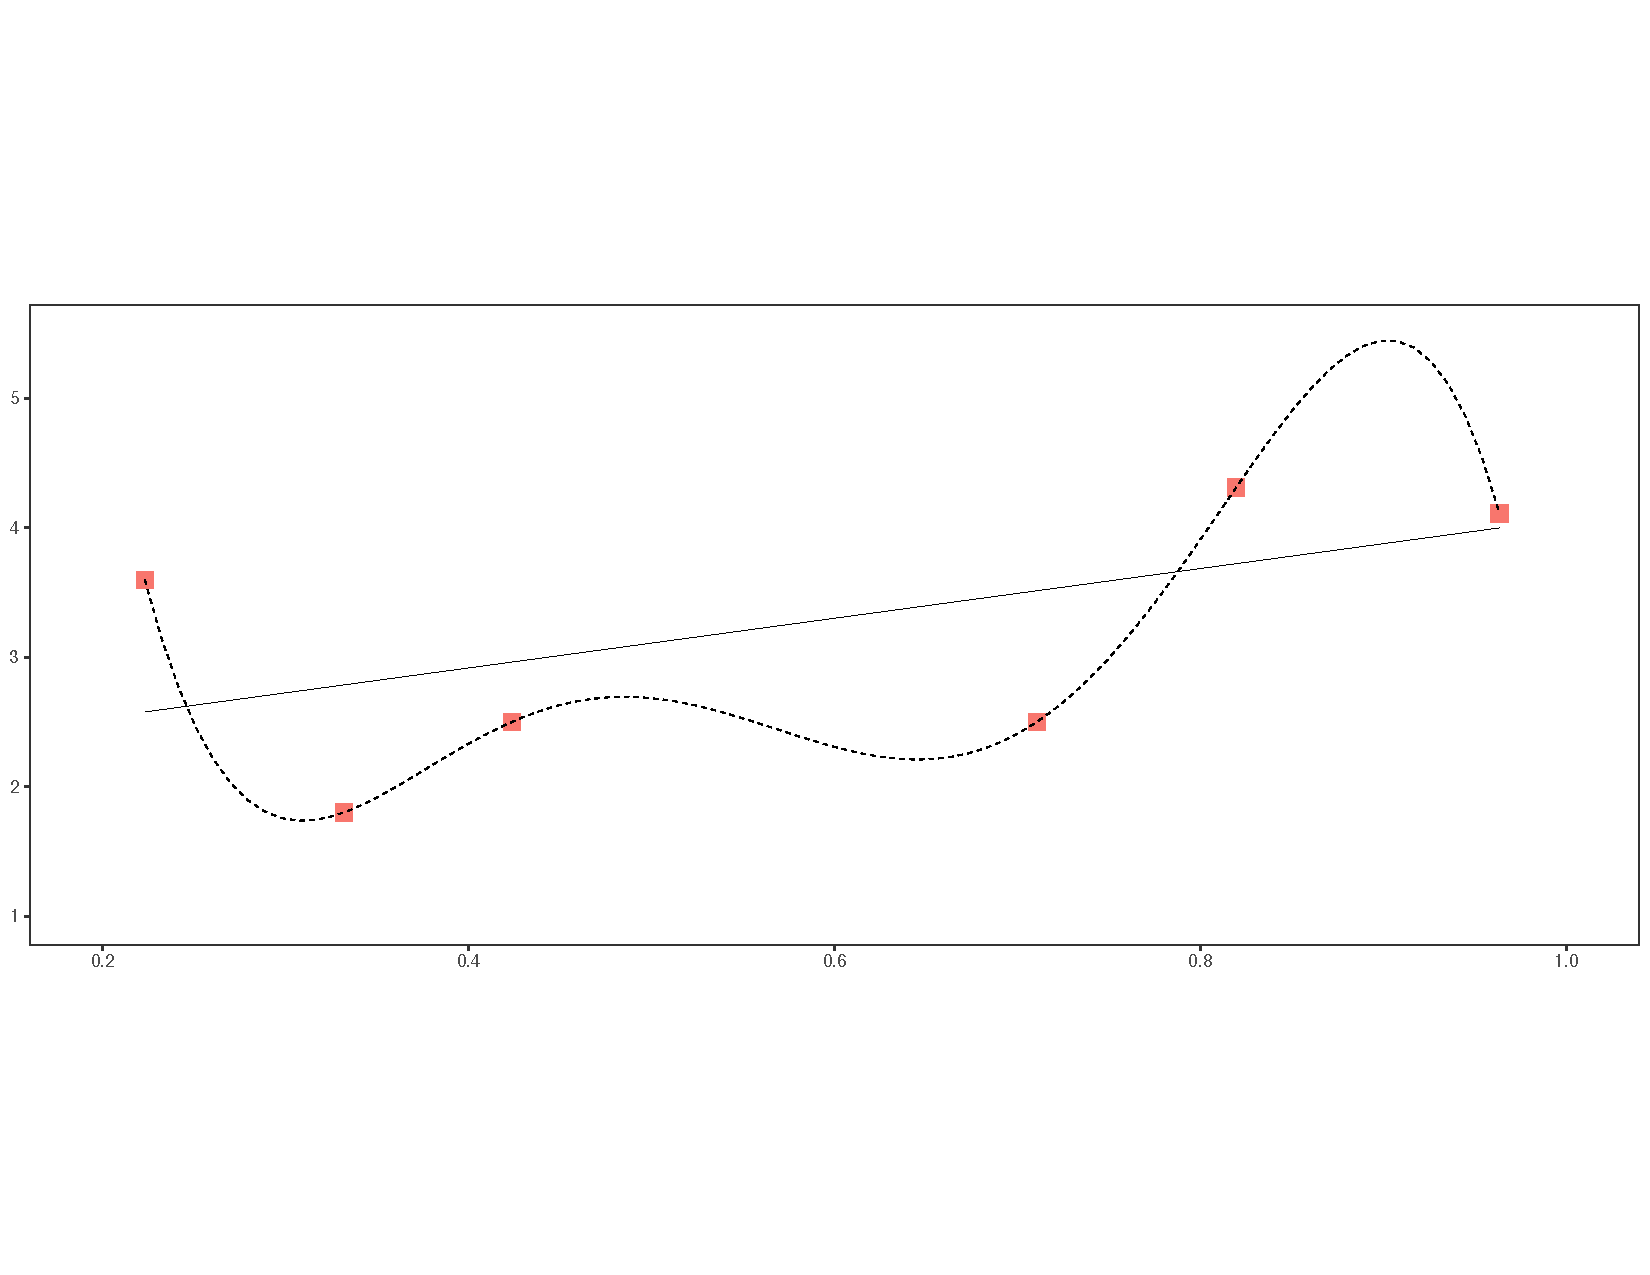
\includegraphics[scale=0.4]{figures/fig_1h_0.pdf}
 \end{figure}


\end{frame}
%----------------------------------------------------------------------%
\begin{frame}[fragile]
\frametitle{Overfit}

\begin{itemize} 
  \item In practice, it doesn't work $\rightarrow$ leads to a terrible out-of-sample fit.
  \item  A deeper answer says that maximal flexibility leaves all the idiosyncratic noise in the prediction model. A new observation with the same x will have a different idiosyncratic noise, and so the prediction is off.
  
\end{itemize}
        \begin{figure}[H] \centering
            \captionsetup{justification=centering}
              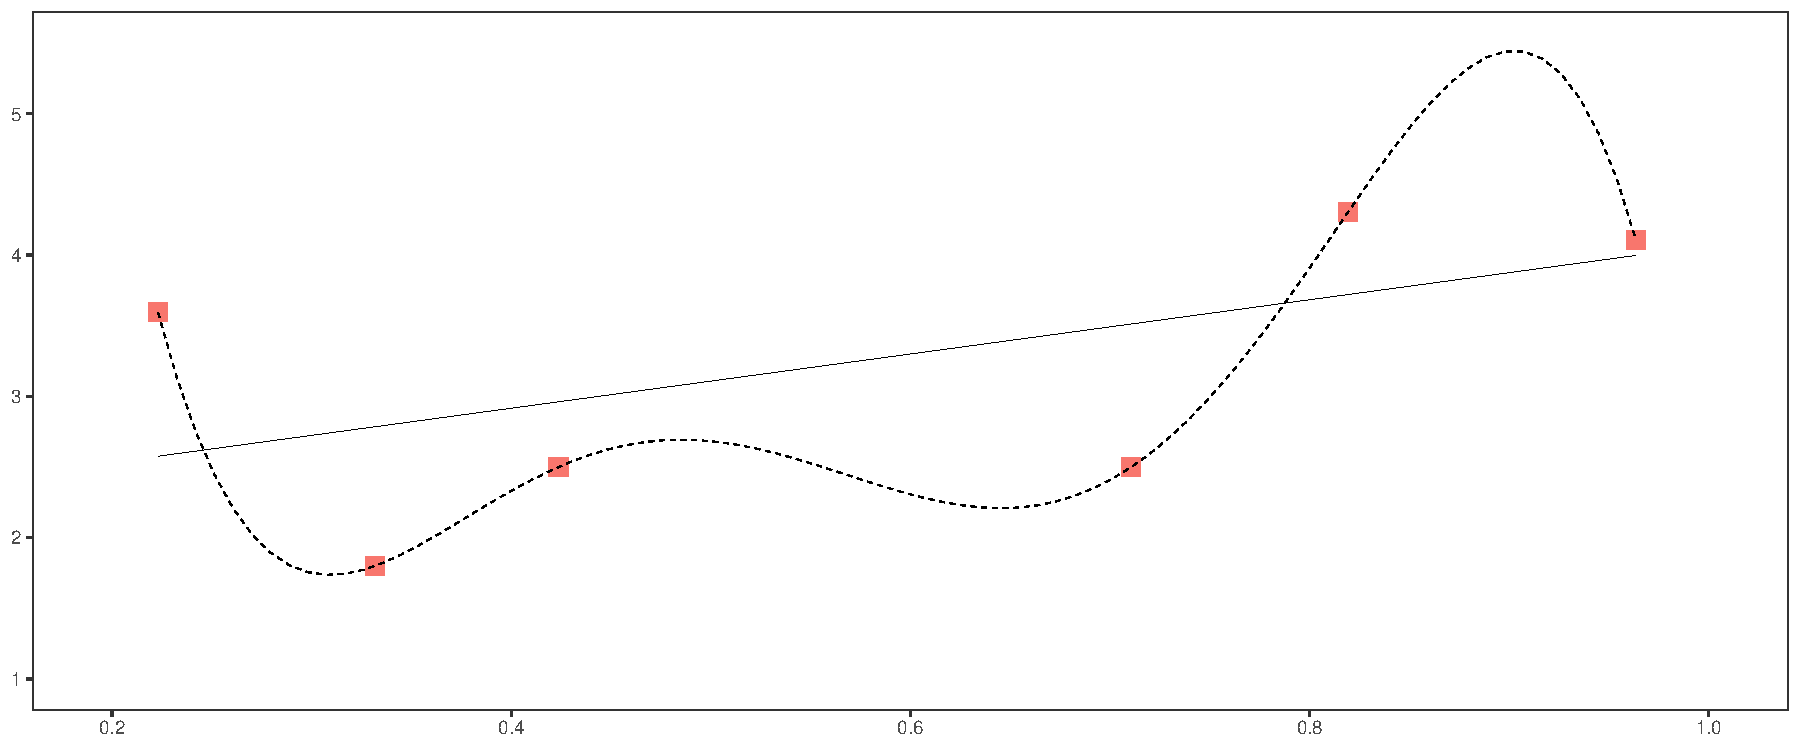
\includegraphics[scale=0.4]{figures/fig_1h.pdf}
 \end{figure}



\end{frame}



%----------------------------------------------------------------------%
\subsection{Overfit and out of Sample Prediction}
%----------------------------------------------------------------------%
\begin{frame}[fragile]
\frametitle{Overfit and out of Sample Prediction}


\begin{itemize}
  \item ML we care about prediction out of sample
  \medskip

  \item To avoid overfitting, we need to find the optimal degree of flexibility.
\medskip
  \item Overfitting is an illustration of the bias-variance trade-off 


\begin{align}
E \left(L(y,\hat{f} \right)  &= E(y-\hat f)^2  \\
                 &= E(f-\hat{f})^2 + E(u^2) \\
                 &=  MSE(\hat f) + E(u^2) \\
                 &=  E(f-\hat f)^2 +E(\hat f-E(\hat f))^2+ E(u^2) \\
                 &= Bias^2(\hat f) + V(\hat f) + E(u^2)
\end{align}

\item Flexibility reduces bias but increases variance. There is an optimal degree of flexibility
  \end{itemize}
\end{frame}
  %----------------------------------------------------------------------%
\begin{frame}[fragile]
\frametitle{Overfit and out of Sample Prediction}


\begin{itemize}

  \medskip
  \item Choose the right complexity level
  \medskip
  \item How do we measure the out of sample error? What is `out of sample'?
  \medskip
  \item $R^2$ doesn't work: measures prediction in sample, it's non decreasing in complexity (PS1)
  \pause
  \medskip
  \item MSE using resampling methods.
\end{itemize}

\end{frame}
%----------------------------------------------------------------------%
\section{Resampling Methods}
%----------------------------------------------------------------------%
\begin{frame}[fragile]
\frametitle{What are resampling methods?}

\begin{itemize}
\item Tools that involves repeatedly drawing samples from a training set and refitting a model of interest on each sample in order to obtain more information about the fitted model
\medskip
\item Model Assessment: estimate test error rates 
\medskip
\item Model Selection: select the appropriate level of model flexibility
\medskip
\item They are computationally expensive! But these days we have powerful computers

\end{itemize}




\end{frame}
%----------------------------------------------------------------------%
\subsection{Validation Set Approach}
%----------------------------------------------------------------------%
\begin{frame}[fragile]
\frametitle{The Validation Set Approach}

\begin{itemize}
\item Suppose that we would like to find a set of variables that give the lowest test (not training) error rate
\item If we have a large data set, we can achieve this goal by randomly splitting the data into training and validation(testing) parts
\item We would then use the training part to build each possible model (i.e. the different combinations of variables) and choose the model that gave the lowest error rate when applied to the validation data
\end{itemize}

       \begin{figure}[H] \centering
            \captionsetup{justification=centering}
              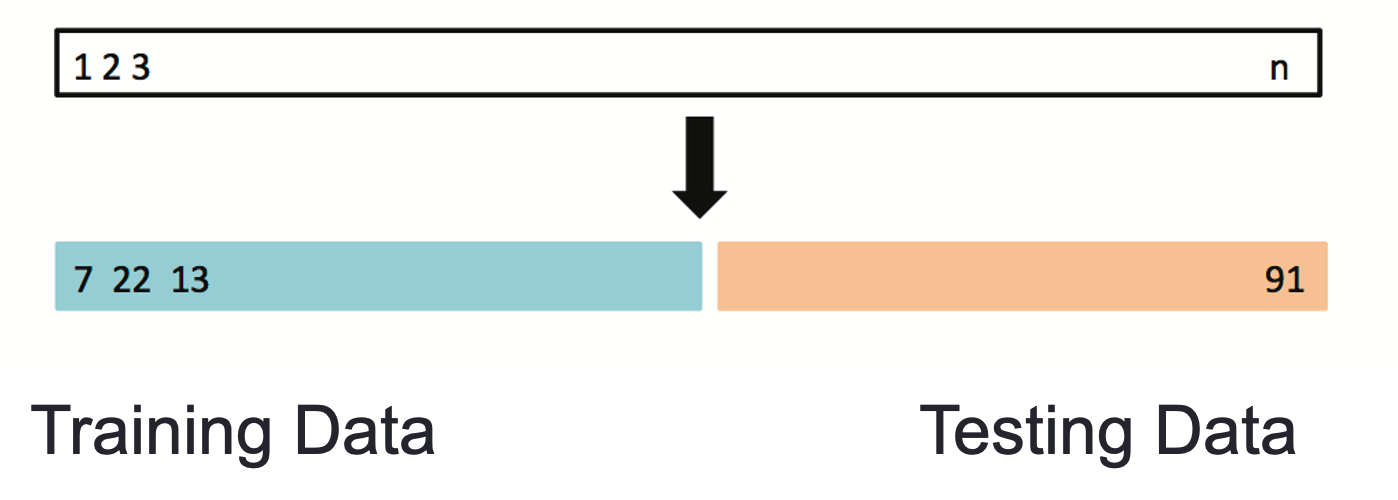
\includegraphics[scale=0.4]{figures/fig51.png}
       \end{figure}

\end{frame}

%----------------------------------------------------------------------%
\begin{frame}[fragile]
\frametitle{The Validation Set Approach}
\begin{itemize}
\item Model $y=f(x) +u$ where $f$ is a polynomial of degree $p^*$. 
\scriptsize
\item Left: Validation error rate for a single split 
\item Right: Validation method repeated 10 times, each time the split is done randomly! 
\item  There is a lot of variability among the MSE’s… Not good! We need more stable methods!
\end{itemize}


 \begin{figure}[H] \centering
            \captionsetup{justification=centering}
              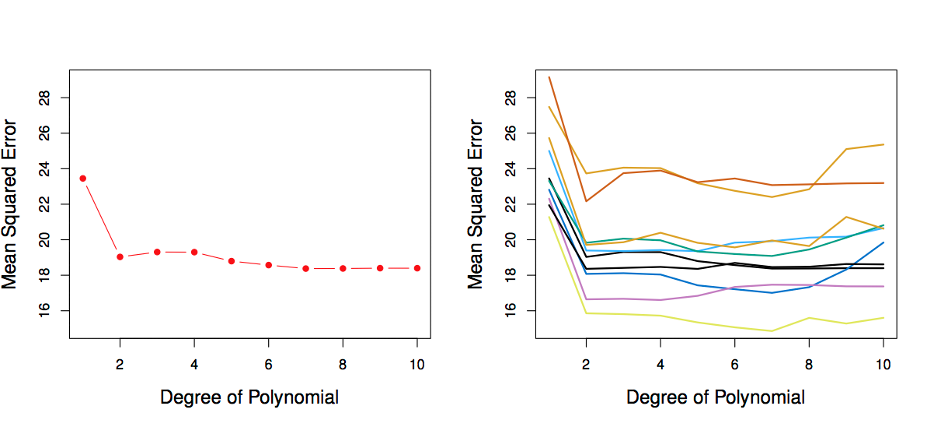
\includegraphics[scale=0.7]{figures/fig52.png}
       \end{figure}
\end{frame}
%----------------------------------------------------------------------%
\begin{frame}[fragile]
\frametitle{The Validation Set Approach}

\begin{itemize}
  \item Advantages:
  \medskip
    \begin{itemize}
      \item Simple
      \medskip
      \item Easy to implement
      \medskip
      \item It may be sensible with really big n
    \end{itemize}
  \item Disadvantages:
  \medskip
    \begin{itemize}
      \item The validation MSE can be highly variable, i.e. , is highly dependent on which observations are included in the testing sample.
      \medskip
      \item Statistical methods tend to perform worse when trained on fewer observations. They have poor small-sample properties; they perform better with increasing sample size. This leads us to overestimate the test MSE.
      
\end{itemize}
\end{itemize}

\end{frame}
%----------------------------------------------------------------------%
\subsection{LOOCV}
%----------------------------------------------------------------------%
\begin{frame}[fragile]
\frametitle{Leave-One-Out Cross Validation (LOOCV)}

\begin{itemize}
\item This method is similar to the Validation Set Approach, but it tries to address the latter’s disadvantages 
\end{itemize}

 \begin{figure}[H] \centering
            \captionsetup{justification=centering}
              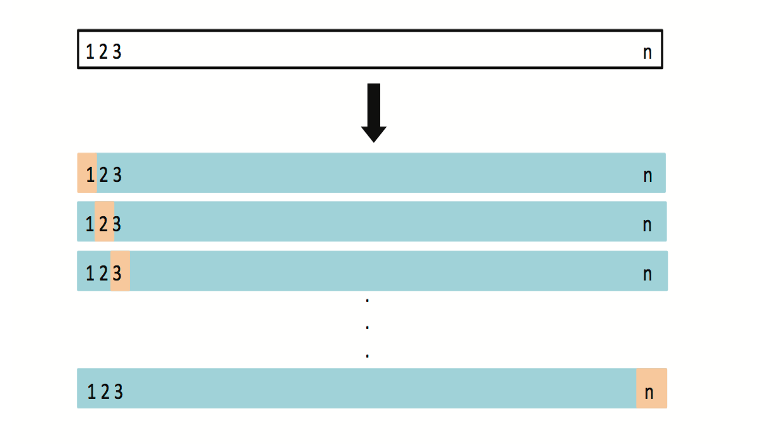
\includegraphics[scale=0.7]{figures/fig53.png}
       \end{figure}


\end{frame}
%----------------------------------------------------------------------%
\begin{frame}[fragile]
\frametitle{Leave-One-Out Cross Validation (LOOCV)}


\begin{itemize}
\item Use a single observation for validation and (n - 1) observations for training.
\medskip
\item Fit the model leaving-one-out observation $\rightarrow \hat{y}_{-i}$.
\medskip
\item Cycle though all n observations
\medskip
\item The LOOCV estimate for the test MSE is
\begin{align}
CV(n) &= n \sum MSE_{-i} \\ 
      &= \frac{1}{n}\sum(y_i -\hat{y}_{-i})^2
\end{align}
\end{itemize}

\end{frame}
%----------------------------------------------------------------------%
\subsection{K-fold Cross-Validation}
%----------------------------------------------------------------------%
\begin{frame}[fragile]
\frametitle{K-fold Cross-Validation}
\begin{itemize}
\item LOOCV is computationally intensive, so we can run k-fold Cross Validation instead
\end{itemize}


 \begin{figure}[H] \centering
            \captionsetup{justification=centering}
              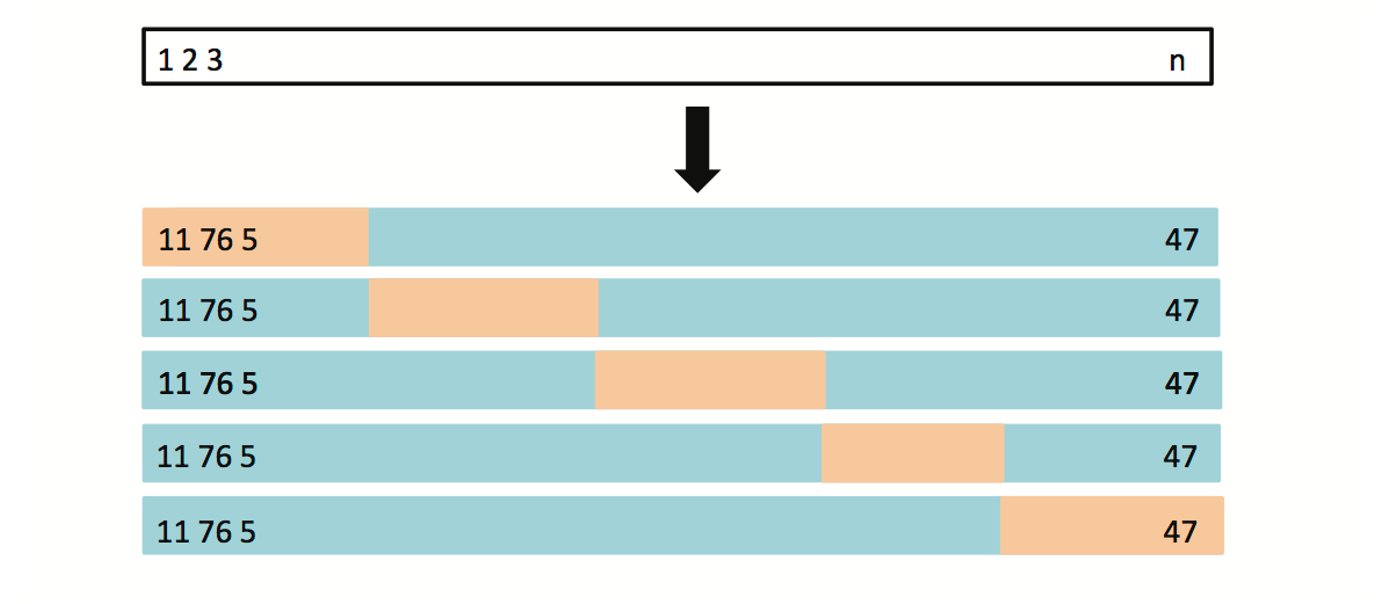
\includegraphics[scale=0.5]{figures/fig55.png}
       \end{figure}



\end{frame}
%----------------------------------------------------------------------%
\begin{frame}[fragile]
\frametitle{K-fold Cross-Validation}

\begin{itemize}
  \item Split the data into K parts $(n=\sum_{j=1}^k n_j)$
  \medskip
  \item Fit the model leaving out one of the folds $\rightarrow$ $\hat{y}_{-k}$
  \medskip
  \item Cycle though all k folds
  \medskip
  \item The CV(k) estimate for the test MSE is


\begin{align}
CV_{(k)} &= \frac{1}{k}\sum_{j=1}^k MSE_j \\
         &= \frac{1}{k}\sum_{j=1}^k (y_j^k-\hat{y}_{-k})
\end{align}
\end{itemize}

\end{frame}
%----------------------------------------------------------------------%
\begin{frame}[fragile]
\frametitle{K-fold Cross-Validation}
\begin{itemize}
  \scriptsize
\item Left: LOOCV  error curve
\item Right: 10-fold CV was run many times, and the figure shows the slightly different CV error rates
\item LOOCV is a special case of k-fold, where k = n
\item They are both stable, but LOOCV (generally) is more computationally intensive! 
\end{itemize}

        \begin{figure}[H] \centering
            \captionsetup{justification=centering}
              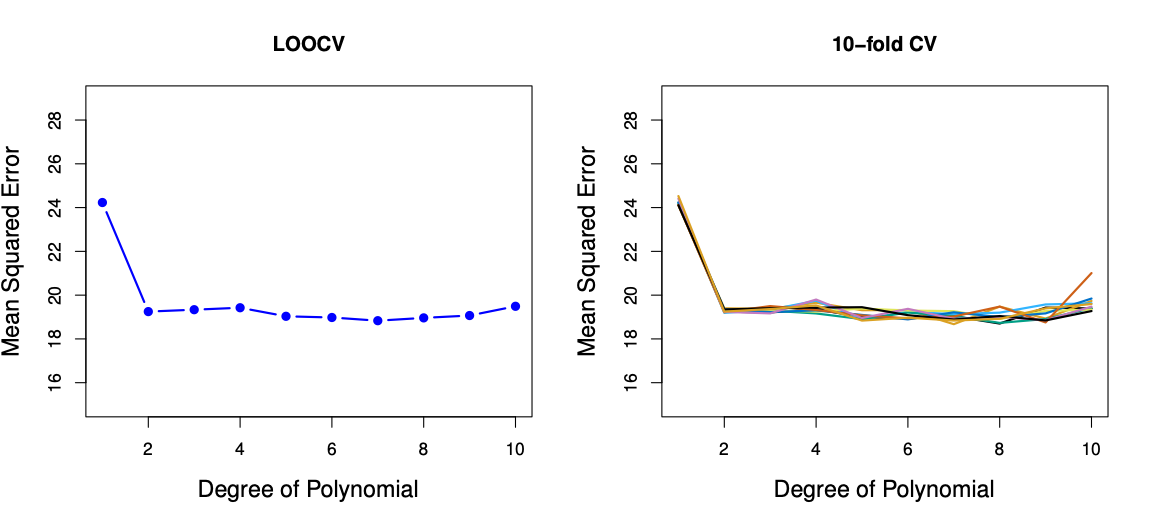
\includegraphics[scale=0.5]{figures/fig54.png}
       \end{figure}
\end{frame}


%----------------------------------------------------------------------%
\begin{frame}[fragile]
\frametitle{Bias- Variance Trade-off for k-fold CV}

\begin{itemize}
  \item Bias:
  \medskip
    \begin{itemize}
      \item Validation set approach tends to overestimate the test error set (less data, worst fit)
      \item LOOCV, adds more data $\rightarrow$ less bias of the test error
      \item K-fold an intermediate state
    \end{itemize}
    \item Variance:
    \begin{itemize}
      \item LOOCV we average the outputs of n fitted models, each is trained in almost identical set of observations $\rightarrow$ highly (positively) correlated
      \item K-fold this correlation is smaller, we are averaging the output of k fitted model that are somewhat less correlated
    \end{itemize}
    \medskip
  \item Thus, there is a trade-off between what to use
  \medskip
    \begin{itemize}
      \item We tend to use k-fold CV with (K = 5 and K = 10)
      \item It has been empirically shown that they yield test error rate estimates that suffer neither from excessively high bias, nor from very high variance Kohavi (1995)
    \end{itemize}
\end{itemize}


\end{frame}



%----------------------------------------------------------------------%
\begin{frame}[fragile]
\frametitle{Spatial K-fold Cross-Validation }

\begin{itemize}
  \scriptsize
  \item 'First law' of geography states that points close to each other are, generally, more similar than points further away
  \item Points are not statistically independent because training and test points in conventional CV are often too close to each other 
  \item To alleviate this problem `spatial partitioning' is used to split the observations into spatially disjointed subsets 
\end{itemize}

 \begin{figure}[H] \centering
            \captionsetup{justification=centering}
              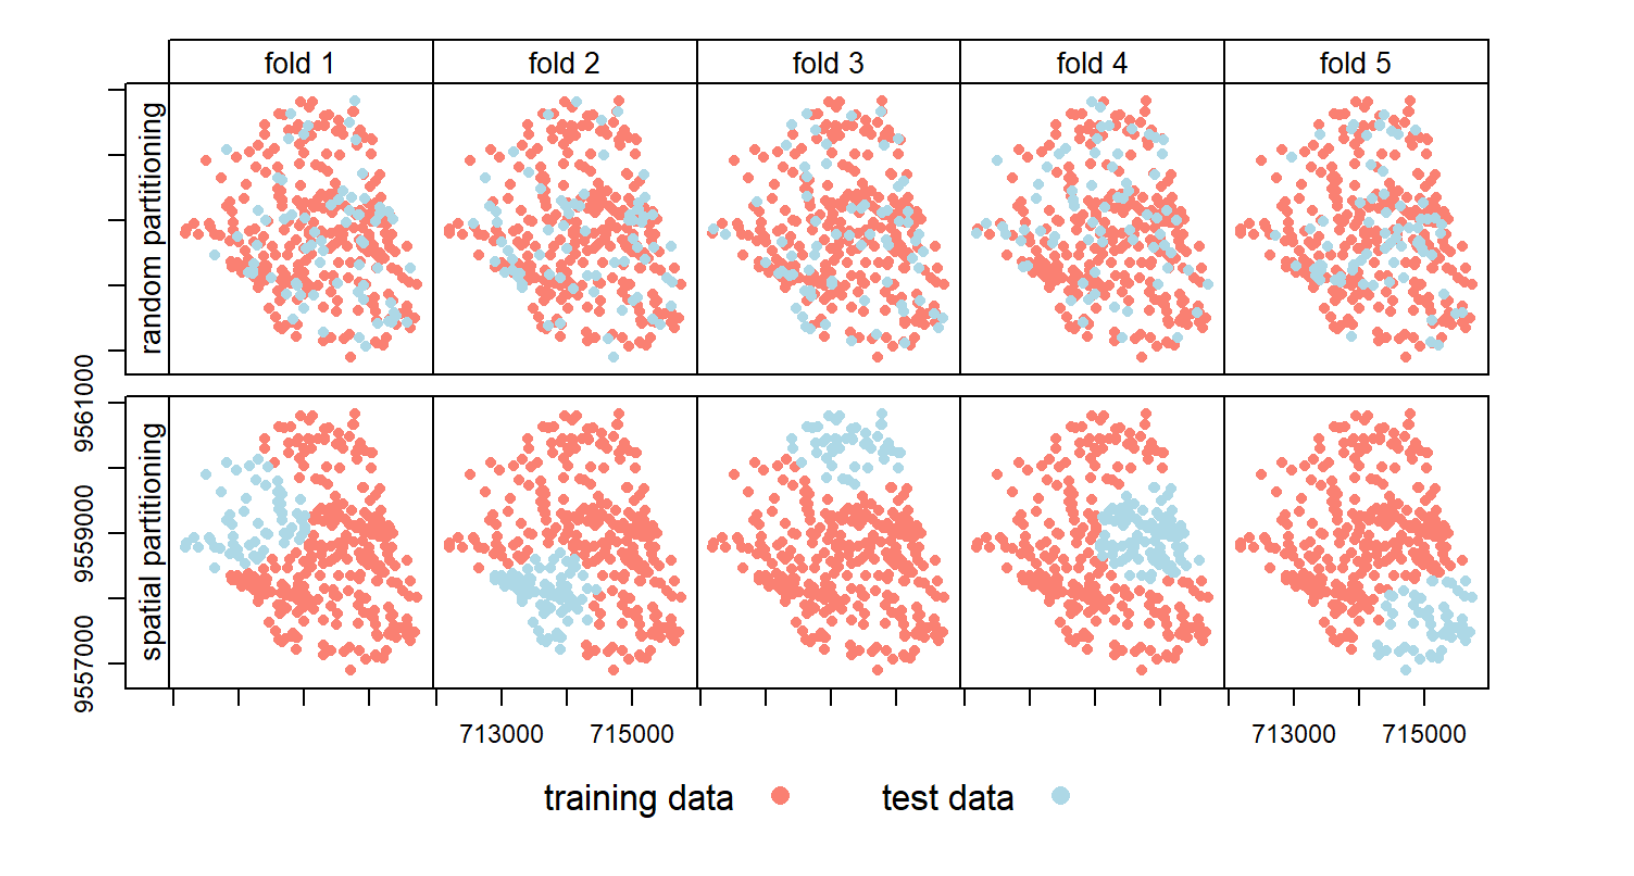
\includegraphics[scale=0.3]{figures/fig113.png}
       \end{figure}

\end{frame}

%----------------------------------------------------------------------%
\begin{frame}
\frametitle{Review \& Next Steps}
  
\begin{itemize} 
    \item Today:
    \medskip
    \begin{itemize} 
         \item Overfit and out of Sample Prediction
         \medskip
         \item Resampling Methods 
        \begin{itemize}  
            \item Validation Set Approach 
            \medskip
            \item LOOCV
            \medskip
            \item K-fold Cross-Validation
      \end{itemize}
    \end{itemize}
  	\bigskip  

	\item  Next class: Model selection and Regularization




\end{itemize}
\end{frame}

%----------------------------------------------------------------------%
\section{Further Readings}
%----------------------------------------------------------------------%
\begin{frame}
\frametitle{Further Readings}

\begin{itemize}


  \item Friedman, J., Hastie, T., \& Tibshirani, R. (2001). The elements of statistical learning (Vol. 1, No. 10). New York: Springer series in statistics.
  \medskip
  \item James, G., Witten, D., Hastie, T., \& Tibshirani, R. (2013). An introduction to statistical learning (Vol. 112, p. 18). New York: springer.
  \medskip
    \item Kohavi, R. (1995). A study of cross-validation and bootstrap for accuracy estimation and model selection. In Ijcai (Vol. 14, No. 2, pp. 1137-1145).
  \medskip
  \item Lovelace, R., Nowosad, J., \& Muenchow, J. (2019). Geocomputation with R. CRC Press. (Chapters 2 \& 6)
\end{itemize}

\end{frame}






%----------------------------------------------------------------------%
%----------------------------------------------------------------------%
\end{document}
%----------------------------------------------------------------------%
%----------------------------------------------------------------------%

